\chapter{Babascriptプログラミング環境の実装}
\label{chap:implementation}

本章では、第\ref{chap:design}章で述べたプログラミング環境について述べる。

\section{Babascriptプログラミング環境}\label{babascriptux30d7ux30edux30b0ux30e9ux30dfux30f3ux30b0ux74b0ux5883}

\subsection{概要}\label{ux6982ux8981}

\subsection{処理手順}\label{ux51e6ux7406ux624bux9806}

\begin{enumerate}
\def\labelenumi{\arabic{enumi}.}
\itemsep1pt\parskip0pt\parsep0pt
\item
  人への命令構文を実行する
\item
  命令がNode-Lindaサーバを経由してクライアントへと配信される
\item
  命令を受け取ったクライアントがユーザに処理を促す
\item
  命令実行者が、処理結果を入力する
\item
  Node-Lindaサーバを経由して実行元プログラムに入力された処理結果が送信される
\item
  プログラム側で指定されたコールバック関数が実行され、処理が継続される
\end{enumerate}

\section{Babascript}\label{babascript}

プログラムと人とのインタラクションを実現するためには、プログラム上で人間への指示を行える仕組みが必要だ。
そこで、Babascriptという、人間への指示構文を実装したオブジェクト(以下、人間オブジェクト)を宣言できるプログラミングライブラリを実装した。
BabascriptはJavascriptのサーバサイド実行環境であるNode.js及びプログラミング言語Ruby上で動作する。

\subsection{基本仕様}\label{ux57faux672cux4ed5ux69d8}

Babascriptでは、通常のメソッド実行とほぼ同じ記法で人間への指示を送ることができる。
例えば、図\ref{fig:babascript_sample}のようなプログラムによって、人間オブジェクトを宣言し、人間へ指示を送ることができる。

\begin{figure}[htbp]
\begin{center}
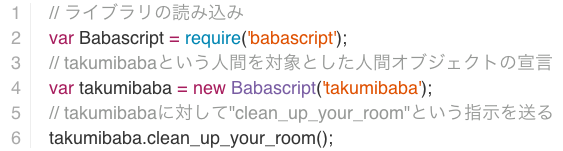
\includegraphics[width=.8\linewidth,bb=0 0 563 151]{images/babascript_sample.js.png}
\end{center}
\caption{人への命令構文}
\label{fig:babascript_sample}
\end{figure}

人オブジェクトはインスタンス生成時にidを指定する必要がある。
人への命令構文は、このidを元に命令配信先を決定する。 例えば、id=baba
に命令を送りたければ、人オブジェクト宣言時の第一引数にはbabaという文字列を指定する。
指定したidに命令が配信されるため、Babascript
Client側でも同じidを指定する必要がある。

人間オブジェクトは、人間オブジェクトに定義されていないメソッドが実行されると、エラーを返さずに、人間への指示として解釈する。
そのため、実装されていないメソッド名であれば、あらゆる命令をメソッドとして表現し実行することが可能である。
例えば、「toString」や「call」等のメソッドは、javascriptにおいてはほぼすべてのオブジェクトが持つメソッドだ。
一方で、「clean\_up\_your\_room」や「bake\_bread」のようなメソッドは定義しない限りは存在しないメソッドである。
Babascriptは、この定義されていないメソッドをエラーとして評価せず、人への命令構文として評価する。

\begin{figure}[htbp]
  \begin{center}
  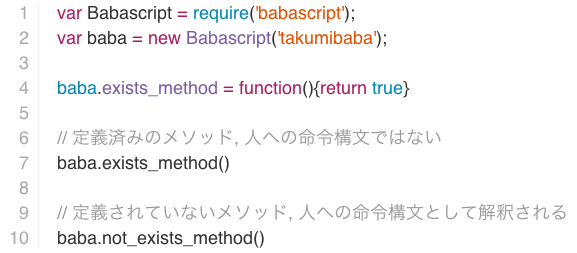
\includegraphics[width=.8\linewidth,bb=0 0 577 330]{images/methodmissing_sample.js.png}
  \end{center}
  \caption{人への命令構文}
  \label{fig:methodmissing_sample}
\end{figure}

オブジェクトに存在しないメソッドが呼び出された時に、特定のメソッドにその処理を委譲するような仕組みは、プログラミング言語Rubyにおいては
methodmissingと呼ばれる。
各言語によって名称は異なるが、類似する仕組みが存在する言語は複数存在する。

人間への指示として評価されたメソッドは、そのメソッド名と引数を元にしたタスク情報を生成し、タスク配信サーバへと送信する。
この際、メソッド名部分がユーザに命令として提示される文となる。
タスク情報は図\ref{fig:task_format}のように構成される。

\begin{figure}[htbp]
\begin{center}
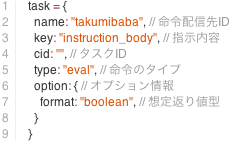
\includegraphics[width=.6\linewidth,bb=0 0 354 225]{images/task_format.js.png}
\end{center}
\caption{タスク情報}
\label{fig:task_format}
\end{figure}

メソッド名が自由に設定できるため、内容は指示ではなく、質問のようなものもあり得るが、本研究では統一して指示と呼ぶ。
人への命令構文の第一引数にはオプション情報を指定する。
第二引数には人力処理の実行後に実行するコールバック関数を指定する。
このコールバック関数は、指示に対して何かしらの値が返されたときに実行される。

\subsection{オプション情報の付加}\label{ux30aaux30d7ux30b7ux30e7ux30f3ux60c5ux5831ux306eux4ed8ux52a0}

メソッド名以外に送信したい情報があるときには、第一引数にオプション情報としてオブジェクトを与える。
クライアントアプリケーション側でオプション情報を得ることができるため、このオプション情報に応じて
ユーザに提示する画面を変更するといったことが可能である。

オプション情報の例としては、返り値の型情報や、タイムアウト情報などが考えられる。
オプション情報は図\ref{fig:babascript_option}のように記述する。
図\ref{fig:babascript_option}の場合であれば、返り値の型はstringで、3分後までに返り値を得られなかった場合は、
人力処理を止め、第二引数で指定するコールバック関数を実行し、処理を続行させるといったことをオプション情報として記述している。

\begin{figure}[htbp]
  \begin{center}
  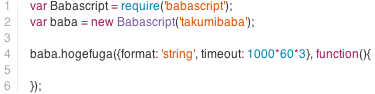
\includegraphics[width=.8\linewidth,bb=0 0 563 149]{images/babascript_option_sample.js.png}
  \end{center}
  \caption{オプション情報のサンプルソースコード}
  \label{fig:babascript_option}
\end{figure}

また、図\ref{fig:babascript_option_list}の場合であれば、listで指定した選択肢の中から選んで返り値を返す、といった指定が可能だ。

\begin{figure}[htbp]
  \begin{center}
  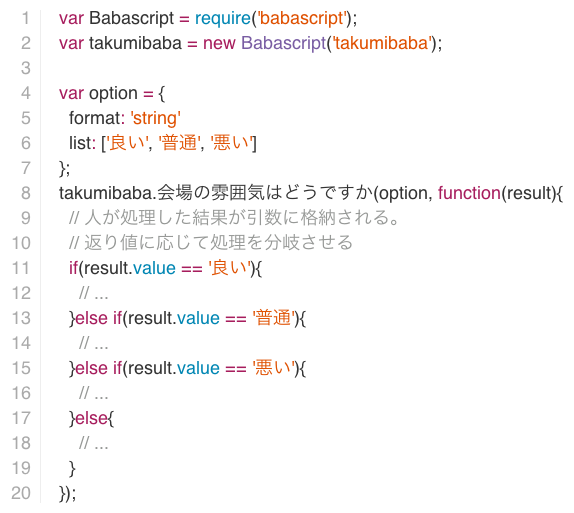
\includegraphics[width=.5\linewidth,bb=0 0 574 513]{images/babascript_option_list.js.png}
  \end{center}
  \caption{オプション情報のサンプルソースコード}
  \label{fig:babascript_option_list}
\end{figure}

オプション情報である第一引数は省略可能である。
省略した場合は、自動的に図\ref{fig:option_default}のようなオブジェクトが代入される。
図\ref{fig:option_default}のオプション情報の場合、返り値の型はBooleanで返すように指定できる。

\begin{figure}[htbp]
  \begin{center}
  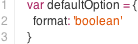
\includegraphics[width=.4\linewidth,bb=0 0 210 70]{images/option_default.js.png}
  \end{center}
  \caption{デフォルトのオプション情報}
  \label{fig:option_default}
\end{figure}

\subsection{コールバック関数の指定}\label{ux30b3ux30fcux30ebux30d0ux30c3ux30afux95a2ux6570ux306eux6307ux5b9a}

命令構文の第二引数にコールバック関数を指定すると、実行結果を取得した後にこのコールバック関数が呼ばれる
resultの中に処理結果が入ってる

人間は計算機の処理に比べて遅延しがちであるため、非同期を前提とした実装をしている

\subsection{コマンドラインでの利用}\label{ux30b3ux30deux30f3ux30c9ux30e9ux30a4ux30f3ux3067ux306eux5229ux7528}

Babascriptはコマンドラインツールとしても利用可能だ。
babaコマンドは、図\ref{fig:baba_command}のように利用することができる。
オプションeの直後に指示内容を、オプションnの直後に指示先のIDを指定する。
format情報などを付加したい場合は、オプションoの後に=の形で指定することができる。

\begin{figure}[htbp]
  \begin{center}
  
\includegraphics[width=.6\linewidth,bb=0 0 465 17]{images/baba_command.sh.png}
  \end{center}
  \caption{Babaコマンド}
  \label{fig:baba_command}
\end{figure}

図\ref{fig:baba_command_pipe}のように、pipeして使うなどの利用方法が考えられる。

\begin{figure}[htbp]
  \begin{center}
  \includegraphics[width=.4\linewidth,bb=0 0 465 17]{images/baba_command_pipe.sh.png}
  \end{center}
  \caption{Babaコマンドでpipeする}
  \label{fig:baba_command_pipe}
\end{figure}

\section{Babascript Client}\label{babascript-client}

Babascriptによって人への指示をプログラムに記述し、実行することが可能となったが、その指示を人に伝え、
処理結果を返させるためのアプリケーションが必要となる。
そこで、Babascript Clientというアプリケーション群を実装した。 Babascript
Clientは、Babascriptとの通信を担うサービス部と返り値の入力等を担うインターフェス部から構成される。
サービス部はJavascript上で動作する。
インタフェース部は、各種アプリケーションに応じて動作環境が異なるが、主にNode.js上とWebブラウザ上で動作する。

\subsection{サービス}\label{ux30b5ux30fcux30d3ux30b9}

サービス部は、主にBabascriptとのやりとり、つまり、命令の受け取りや返り値の送信などを担う。

命令を受け取ると、イベントを発行する

\begin{figure}[htbp]
  \begin{center}
  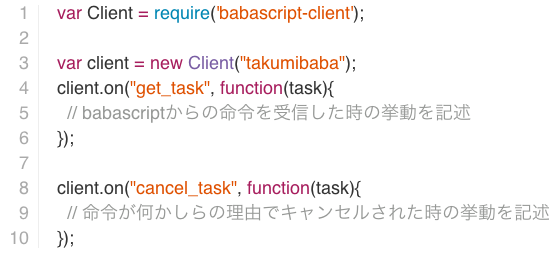
\includegraphics[width=.8\linewidth,bb=0 0 560 253]{images/babascript_client_service.js.png}
  \end{center}
  \caption{Babascript Client サービス部}
  \label{fig:babascript_client_service}
\end{figure}

何かしらの値を実行結果として返すときは、clientオブジェクトに実装されているretrnValueメソッドを用いる。
図\ref{fig:babascript_client_service_returnvalue}のように、第一引数に結果として返すものを指定する。

\begin{figure}[htbp]
  \begin{center}
  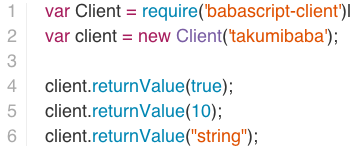
\includegraphics[width=.8\linewidth,bb=0 0 357 149]{images/babascript_client_service_returnvalue.js.png}
  \end{center}
  \caption{Babascript Client 処理結果を返すメソッド}
  \label{fig:babascript_client_service_returnvalue}
\end{figure}

\subsection{ユーザインタフェース}\label{ux30e6ux30fcux30b6ux30a4ux30f3ux30bfux30d5ux30a7ux30fcux30b9}

ユーザとのインタラクションを行う。
命令をユーザに見せるのと、実際に実行結果を入力させる機能を持つ

サービス部と独立した実装のため、異なるデバイスや環境上でもインタフェース部を実装するだけでBabascript
Clientは構築可能である。
基本的には、指示内容と返り値の入力インタフェースをユーザに提示し、返り値の入力を受け付ける機能を担う。
この際、Babascriptの指示でオプション情報として返り値の型を指定していた場合、指定した型以外の入力を受け付けないような実装を行っている。
返り値の型は現在、Boolean, String, Numberに対応している。

例として、Webアプリケーション、コマンドライン・インタフェース、slackインタフェースを実装した。

\subsection{Webアプリケーションインタフェース}\label{webux30a2ux30d7ux30eaux30b1ux30fcux30b7ux30e7ux30f3ux30a4ux30f3ux30bfux30d5ux30a7ux30fcux30b9}

インタフェースの例として、Webアプリケーションとして実装した。
webブラウザ上で動作し、フレームワークにはBackbone.jsとMarionette.jsを利用した。
CSSはLESSを、HTMLはJadeで記述した。 Heroku上で稼働している。

システムは図\ref{fig:babascript_client_webapp}のように構成される。

\begin{figure}[htbp]
  \begin{center}
  \includegraphics[width=.3\linewidth,bb=0 0 273 402]{images/babascript_client_webapp_system.png}
  \end{center}
  \caption{Babascript Client Slackインタフェース}
  \label{fig:babascript_client_webapp_system}
\end{figure}

Webインタフェースでは、指示内容に応じて提示インタフェースを変化させる実装をしている。
例えば、フォーマットにBooleanを指定していた場合、ユーザには trueボタンと
falseボタンが提示され、
どちらかのボタンを押すと、その結果が返り値としてプログラムに返される。
また、StringとNumberであれば、文字・数字の入力フォームと投稿ボタンが提示され、
投稿ボタンを押した際にフォームに入力されていた内容が返り値としてプログラムに返される。
実際に提示されるインタフェースの例を図\ref{fig:babascript_client_webapp_interface}に示す。

\begin{figure}[htbp]
\begin{center}
\includegraphics[width=.3\linewidth,bb=0 0 273 402]{images/babascript_client_webapp_interface.png}
\end{center}
\caption{Babascript Client Slackインタフェース}
\label{fig:babascript_client_webapp_interface}
\end{figure}

\subsection{CommandLineインタフェース}\label{commandlineux30a4ux30f3ux30bfux30d5ux30a7ux30fcux30b9}

\subsection{チャットボットインタフェース}\label{ux30c1ux30e3ux30c3ux30c8ux30dcux30c3ux30c8ux30a4ux30f3ux30bfux30d5ux30a7ux30fcux30b9}

チャットサービス上で稼働するボットにBabascript Clientの機能を実装した。
ボットシステムにはHubotを採用した。
Hubotは様々なチャットサービスに対応しているが、Slackというチャットサービス上において運用している。
このボットシステムは、Heroku上で稼働している。
チャットボットのシステム図を図\ref{fig:babascript_client_hubot_system}に示す。

\begin{figure}[htbp]
  \begin{center}
  \includegraphics[width=.3\linewidth,bb=0 0 273 402]{images/babascript_client_hubot_system.png}
  \end{center}
  \caption{Babascript Client Slackインタフェース}
  \label{fig:babascript_client_hubot_system}
\end{figure}

チャットボットシステムは、ユーザからのメッセージによる問い合わせに応じて返答を行う。
返答の例を図\ref{fig:babascript_client_slack}に示す。

\begin{figure}[htbp]
  \begin{center}
  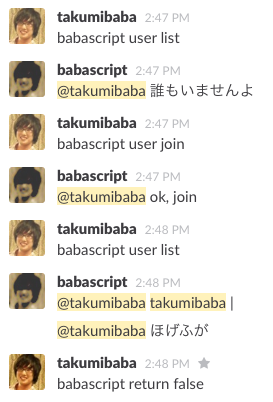
\includegraphics[width=.3\linewidth,bb=0 0 273 402]{images/babascript_client_slack.png}
  \end{center}
  \caption{Babascript Client Slackインタフェース}
  \label{fig:babascript_client_slack}
\end{figure}

チャットボットシステムの問い合わせに対する動作のリストを表\ref{tb:babscript_hubot_mention}に示す。

チャットボットインタフェースでは、Webアプリケーションの場合と違い、
提示するインタフェースを返り値の型に応じて変化させるといったことができない。
そのため、ユーザにとっては値を返しにくくなっているが、普段利用しているチャットサービス上で
Babascript
Clientの機能を利用できるということは有用なことであると考える。

\section{通信手法}\label{ux901aux4fe1ux624bux6cd5}

BabascriptとBabascript
Client間のデータ通信には、Node-LindaというWebサービスを利用する。
Node-Lindaは、分散並列処理のための仕組みであるLindaをNode.js上に実装したものである。
Node-Lindaはネットワーク経由のデータ通信を前提としており、複数の通信手法に対応している。
本研究では、デバイスごとに利用可能な通信手法が異なるという状況を想定したものである。
そこで、このNode-Lindaに接続するための複数のAdapterを実装した。
このAdapterは簡単に切り替えることができ、各実装に影響を与えることがないよう設計されている。
Babascript及びBabascript
Clientは双方共にこのAdapterを利用して通信を行う。

具体的にはSocket.IO AdapterとPush Notification Adapterの2つを実装した。
以下の節で具体的に述べる。

\subsection{Node-Linda}\label{node-linda}

Node-Lindaについて どのようなタプルを書くのか take, watch, read,
writeについて

\subsection{Socket.IO Adapter}\label{socket.io-adapter}

Socket.IO
Adapterは、リアルタイム通信のためのライブラリであるSocket.IOを用いてNode-Lindaに接続するためのAdapterだ。
WebsocketもしくはXHR-Pollingによって常にNode-Lindaサーバと通信を行い続ける。
常時通信している都合上、バッテリー消費の問題が生じたり、デバイスによっては通信を強制的に切断されてしまうこともある。

構成図を図\ref{fig:socket.io-adapter}に示す。

\subsection{PushNotification Adapter}\label{pushnotification-adapter}

Pushnotification Adapter は、HTTP
RequestとPushNotificationを用いてNode-Lindaと通信を行うためのAdapterだ。
Node-Lindaへのタプル書き込みや処理待ちの登録にはHTTP Requestを投げる。
Node-Linda側からAdapter側への通信には、PushNotificationを用いる。
現在は、Amazon AWS
SimpleNotificationServiceを利用し、PushNotificationを実現している。
主にAndroidやiPhone等のモバイルデバイスからNode-Lindaと接続する際に利用する。

構成図を図\ref{fig:pushnotification-adapter}に示す。

\section{プラグイン機構}\label{ux30d7ux30e9ux30b0ux30a4ux30f3ux6a5fux69cb}

Babascript
及びBabascriptClientはその機能を拡張するために、プラグイン機構を持つ。

図\ref{fig:babascript_plugin}の様に使うことで、Babascript及びBabascriptClientによってイベントが発生した時に、
それに応じたデータを受け取り、自由に操作することができる。

\begin{figure}[htbp]
  \begin{center}
  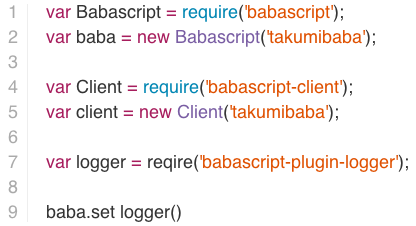
\includegraphics[width=.7\linewidth,bb=0 0 416 226]{images/babascript_plugin.js.png}
  \end{center}
  \caption{Babascript Plugin}
  \label{fig:babascript_plugin}
\end{figure}

Babascript及びBabascriptClientは、以下のイベントを受け取る。
また、イベントを受け取った際にはイベントに応じたデータを受け取る。

\begin{itemize}
\itemsep1pt\parskip0pt\parsep0pt
\item
  initialize
\item
  connect
\item
  send
\item
  receive
\end{itemize}

initializeイベントは、プラグインが読み込まれた際に発生する。
例えば、設定ファイルの読み込みなどの処理を行う。
connectイベントは、Babascript及びBabascript
ClientがNode-Lindaサーバに接続した際に発生する。
sendイベントは、Babascript及びBabascript
Clientが何かしらのデータをNode-Lindaサーバに書き込む際に発生する。
例えば、指示内容を全てログとして保存したいときなどには、sendイベントと共に受け取るデータを送信するといったことができる。
receiveイベントは、Babascript及びBabascript
Clientが何かしらのデータをNode-Lindaサーバから受け取る際に発生する。
指示を送ってから値が帰ってくるまでの時間を計測したいときなどは、このイベントをフックするプラグインを実装する必要がある。

\subsection{具体例}\label{ux5177ux4f53ux4f8b}

例えば、以下のようなプラグイン例が考えられる。

\begin{itemize}
\itemsep1pt\parskip0pt\parsep0pt
\item
  LoggingPlugin
\item
  DatasyncPlugin
\item
  WearableDevicePlugin
\end{itemize}

\subsubsection{Logger Plugin}\label{logger-plugin}

LoggerPluginは、

\subsubsection{Datasync Plugin}\label{datasync-plugin}
